\documentclass[
a4paper,
12pt,
notitlepage,
parskip=half,
DIV=11,
]{scrbook}

\usepackage[utf8]{inputenx}
\usepackage[T1]{fontenc}
\usepackage{hyperref}
\usepackage{graphicx}

\usepackage[numbers]{natbib}
\usepackage{cite}

\usepackage{tikz}
\usepackage{pgfplots}
\usepackage{color, colortbl}
\definecolor{LightGreen}{rgb}{0.83, 0.91, 0.83}
\definecolor{LightYellow}{rgb}{1.0, 0.95, 0.8}
\definecolor{LightRed}{HTML}{F8CECC}

\definecolor{findOptimalPartition}{HTML}{D7191C}
\definecolor{storeClusterComponent}{HTML}{FDAE61}

\input{genode-manual/manual/img/tikz-preamble.tex}
\input{genode-manual/manual/img/tikz-common.tex}

\renewcommand{\labelenumi}{R\arabic{enumi}}

\begin{document}
	
	\tableofcontents
	
	\chapter{Introduction}
		
	
        At the present time we are surrounded by devices that run complex software and operating systems.
		The number of these devices is still rising and their complexity is growing by the increasing amount computational resources, functionalities and interfaces.
		Also many of these devices are taking over important tasks such as smart locks or even cardiac pacemakers.
		Since most of these devices are connected to the public Internet they cannot only be accessed by their owners but anyone.
		
		Most of the modern systems run on kernels built in a monolithic manner.
		This implies that a high amount of the critical functionality such as device drivers and networking stack are implemented by them.
		All these complex software constructs run on the so called kernel mode which is the highest privileged mode it can achieve.
		It is where the operating system kernel usually runs in.
		Since it can access and control the whole system including any user processes a single vulnerability in any of its components could compromise the entire system.
		
		Furthermore the quality of this software is often bad.
		This is especially true for device drivers which have, according to \citep{Chou:SOSP:01},  around three to seven times higher error rates than other kernel parts.
		That is even more problematic since drivers also are the majority of the code.
		While an attacker often needs to find only a single error monolithic kernels often contain thousands of them due to their large code base.
		
		Also when bugs appear in the kernel it needs in average far over one year until a fix is available.
		And even then it takes additional time until it is brought to the user.
		There are also systems that cannot be patched for different reasons.
		These will stay vulnerable for their whole lifetime. \citep{Chou:SOSP:01}
		
		A first step to mitigate this problem would be the usage of user level drivers.
		The user level is a less privileged mode than the kernel mode.
		It runs most of the software on a system including all conventional end user applications.
		Also while the kernel is able to access any resource like physical memory a process running in the user mode cannot.
		It is limited to its own address range in memory and can access other resources only through the kernel.
		This would not solve the problems based on the errors in the software itself but it would lower their privileges.
		A compromised driver would not be able to access and control the whole system but only a part of it.
		
		Unfortunately user space drivers on Linux are quite uncommon.
		While some approaches exist, such as FUSE \citep{fuse} or Userspace IO (UIO) \citep{uio} they are still limited.
		UIO for example requires a loadable kernel module for each driver which still adds complexity to the kernel instead of taking it away.
		FUSE only implements file system drivers and does not have access to any hardware resources.
		
		A solution to this problem are microkernels.
		They implement only the minimally required functionality inside the kernel which reduces their complexity.
		This includes the management of memory and hardware access.
		They do not implement drivers which are responsible for a high amount of the complexity and errors in monolithic systems. \citep{Chou:SOSP:01}
		
		Based on microkernels drivers are implemented in the user space.
		This lowers their privileges and isolates them from each other.
		The Genode OS Framework is an implementation of this concept. 
		It is a component based system that runs on different microkernels such as NOVA or seL4.
		It realizes a strict separation of its components and only allows a defined communication between them.
		
		Micro kernels often do not support less used or exotic platforms.
		Porting them to a new unsupported platform requires a high effort and needs time.
		Linux however often supports them well and is the only choice for some of them.
		It also comes with good debugging facilities which is an important part for driver development.
		
		The goal of this thesis is the combination of the advantages of both Linux and Genode.
		While it already runs on Linux there is no support for hardware access and device drivers yet.
		After stripping away its kernel drivers Linux still has a high complexity.
		Despite this running them in the user space on Genode gains security through isolation while keeping the good platform support.
		
	\chapter{Background}

		\section{Monolithic kernels}
		
		The kernel is an operating systems most crucial part.
		It controls access to the hardware and manages resources.
		Since it runs with the highest privileges the whole systems security depends on it.
		Most of the widely used operating systems rely on so called monolithic kernels.
		Well known examples are Linux and Microsoft Windows.
		
		A monolithic kernel implements many drivers and subsystems in the kernel space.
		This extensive functionality introduces a high complexity with, in the case of Linux, multiple millions lines of code \citep{journals/jss/IsraeliF10}.
		The whole code is compiled into a single binary that runs in one address space.
		Within this there exists no isolation between subsystems.
		On one hand this introduces a good performance.
		A complex data structure such as a linked list for example can be passed between subsystems by only sharing the pointer to it.
		Otherwise it would be required to deserialize, copy and the serialize it which comes with relevant overhead.
		On the other this introduces vulnerabilities since a single compromised subsystem can access anything else in the kernel.
		
		An example for this is a vulnerability in a Synaptics touchscreen driver.
		In this case which emerged in 2017 on Android it is possible escalade execution privileges to the kernel space from the driver process.
		This leads to a full compromise of the whole kernel by allowing code execution in the kernel space.
		The attacker is then able to read any data from the device including passwords and files on the internal storage and execute any code to manipulate network traffic for example. \citep{cve-2017-0581}
		
		Figure \ref{monolithickernel} shows the large complexity that monolithic kernels incorporate.
		Anything in the orange marked area is running inside the kernel and therefore in a single address space with no isolation.
		This also counts for loadable kernel modules.
		In contrast to their naming they are not modularized from the kernel.
		They run in the same address space and have the same privileges as the rest of the kernel.
		This is even more critical since they can be proprietary.
		
		To interface with the user space a monolithic kernel uses so called syscalls.
		These are defined procedures that can be called from the user space to do tasks that require the kernel.
		This could be simply opening a file but also mapping I/O memory and manipulating hardware.
		When a system call is used, its parameters are put on the stack and a so called trap is executed.
		This triggers a mode switch into the kernel space where the arguments are taken from the stack and the according operation is executed. \citep{Tanenbaum2001}
		
		Yet due to the high amount of functionality there are plenty of system calls.
		The Linux kernel counts, depending on the version, between 350 \citep{journals/jss/IsraeliF10} and nearly 400 \citep{syscalls} of them.
		This introduces a high complexity and a large attack surface.
		
		
		\begin{figure}
			\centering
			\def\svgwidth{0.8\textwidth}
			\input{monolithic.pdf_tex}
			\caption{Monolithic kernel system architecture}
			\label{monolithickernel}    
		\end{figure}
		
		\section{Microkernels}
		
		Micro kernels aim to implement as few functionality as possible inside the kernel.
		Their task is to isolate user space components from each other.
		The kernel implements message passing mechanisms to allow communication between these and enforces policies that describe the allowed routes of communication.
		This aims to make the system highly modularizable and isolate failures in components from the rest of the system.
		
		Micro kernels are used on embedded chips.
		Apples A-Series processors contain a coprocessor called Secure Enclave.
		It is responsible for cryptographic operations and key management and has to maintain the protection of the keys even if the system running on the application processor is compromised.
		It uses a customized version of the L4 microkernel \citep{ios11sec} \citep{Heiser:2016:LML:2912578.2893177}.
		
		Although virtualisation is often associated with large scaled servers it is also used on embedded devices.
		In this context micro hypervisors such as NOVA \citep{Steinberg:2010:NMS:1755913.1755935} are used.
		These are specialized microkernels that make use of the virtualisation technologies available on many platforms to run multiple systems isolated from each other. \citep{ibmvirt}
		
		As a general requirement a microkernel should only functionality that would be infeasible to implement outside the kernel.
		It also has to separate and protect applications from itself and each other.
		Any component that runs on a microkernel must not be influenced by any other. And if two components communicate between each other the communication must be secure in regards of confidentiality and integrity.
		
		To fulfil these requirements a microkernel based system consists of tasks that run in the user space.
		As shown in figure \ref{microkernel} they are isolated from each other but can communicate via IPC with each other and the kernel.
		Each task owns an address space which only itself can access.
		Since they cannot influence each other the goal of isolation is satisfied.
		Any communication between them is done via IPC or well defined shared memory regions.
		
		A task is a process that is characterized through its own state including its address space, stack pointer and instruction pointer.
		Any changes the thread applies to its address space are controlled by the kernel.
		Yet it is able to create a child that can inherit parts of its resources.
		The parent looses access to anything it grants to the child regains it once the it is terminated.
		Since the child itself can spawn new children a tree like structure can emerge.
		
		Address spaces are mappings from physical to virtual memory pages.
		The kernel takes a page of physical memory and assigns it to a task.
		The assigned pages get their own address range each making this process transparent to the task.
		Figure \ref{mapping} shows that each task only can see its virtual addresses and does know neither which physical memory it possesses nor where other tasks are located.
		The assignment and management of these mappings is done by the kernel.
		
		If a task spawns a child it passes a part of its own resources to the child.
		It also looses access to this memory.
		In figure \ref{mapping} the first task spawns a child which gets the parents second half of the memory.
		The child itself cannot conclude from this to the physical or its parents memory location and size.
		If the parent wants to keep the space it has passed to its child, for example to employ shared memory, it can map it to the child.
		To reverse the mapping the according address space can be flushed removing it from all other subsystems except the flushing one.
		The management of the resources that are affected by these operations is done in the kernel itself.
		While I/O memory is a does not necessarily represent physical main memory it is also managed in this context.
		
		\begin{figure}
			\centering
			\def\svgwidth{0.8\textwidth}
			\input{mapping.pdf_tex}
			\caption{Mapping physical to virtual memory}
			\label{mapping}    
		\end{figure}
		
		Inter process communication (IPC) is a defined way for two threads to communicate with each other.
		While both parties must agree to the transmission the sender controls the content while the receiver has to handle it.
		This handling includes how the content is interpreted and if it is used at all.
		
		Remote procedure calls (RPC) can call procedures in another task.
		When such a call is done the arguments are sent to the executing task which then does its computation.
		Once the result is available it is returned to the sender.
		On the senders side the call blocks execution until the result is available.
		The passing of arguments and result is usually done via IPC.
		
		Interrupts are an often used way of devices to notify the software of events.
		This mechanism also needs to be supported on microkernels.
		Interrupts can be implemented by empty IPC messages which are sent from threads that have special ids.
		These map to hardware interrupt ids.
		The receiving thread can conclude to the triggered interrupt by the source id \citep{Liedtke_1995}.
		On more recent system such as NOVA interrupts can be implements as semaphores for example \citep{Steinberg:2010:NMS:1755913.1755935}.
		
		\begin{figure}
			\centering
			\def\svgwidth{0.8\textwidth}
			\input{micro.pdf_tex}
			\caption{Micro kernel system architecture}
			\label{microkernel}    
		\end{figure}
		
		\section{Genode}
		
		The Genode OS framework is the implementation of this architecture for highly secure special purpose operating systems.
		Mainly written in C++ it scales from embedded systems with only a few megabytes of memory to big systems with dynamic workloads.
		It implements all applications and drivers as user space components and provides isolation between them.
		
		User space applications in Genode are managed by capabilities.
		They provide a way to allow and deny access to system resources such as RAM or I/O memory without the need for a global complex policy.
		Additionally to capabilities resources can be managed in a hierarchical way.
		Software components can be be partitioned into parts of different complexity.
		This helps to exclude complex parts from the trusted computing base and therefore reduce the amount of code that needs to be verified.
		The continuation of this approach leads to an application specific trusted computing base that consists of the application itself and all the parts it depends on [\ref{fig:tcb_tree}].
		\citep{genode}
		
		\begin{figure}
			\centering
			\input{genode-manual/manual/img/app_specific_tcb.tikz}
			\caption{Application based TCB \citep{genode}}
			\label{fig:tcb_tree}
		\end{figure}
		
		The architecture consists of a recursive sandbox structure.
		Those are controlled from their parents and separated from their siblings.
		But they can create additional sandboxes and subtrees of children.
		This creates hierarchical structures and reduces the attack surface of the system since a compromised component cannot access resources of other components.
		These components are small blocks that can create complex systems without unnecessarily increasing the trusted computing base.
		Beside being programs they can also provide other functionalities such as device drivers or protocol stacks.
		
		Genode supports multiple CPU architectures such as Intel i386 and ARM.
		Multiple microkernels such as NOVA and seL4 can be used.
		Additionally Genode provides a custom kernel implementation that in comparison to other kernels further reduces the trusted computing base.
		The current framework also provides many usable driver and application components.
		Beside common periphery drivers such as USB and Intel wireless this also includes complex application frameworks such as Qt5. \citep{genode}
		
		To debug components in the development process Genode can also be started on the current running Linux kernel.
		This is a good approach for applications but is also limited.
		Some resources cannot be used since the Linux kernel doesn't provide them to the user space, for example memory mapped IO or direct memory access.
		To develop and debug native Genode device drivers the kernel needs to act as a microkernel and provide access to these resources in Genode.
		
		Some of Genodes properties are important for the evaluation of this thesis and will be explained further.
		One is the source code management which is based on so called repositories that can include multiple sets of software components.
		The other is the session concept which implements the IPC mechanism and also provides abstractions to platform specific code.
		
		\subsection{Components}
		
		Genode based systems are based on components.
		These can be drivers, services, applications.
		Their public interface to other components is defined by the sessions they require and provide.
		Beside these sessions they are isolated from each other.
		Components do not have any information about their communication partners but only about the type of the sessions they use.
		This type information is provided by a capability that a component needs to use it.
		Due to this property the can be replaced transparently by other components providing or using the same sessions. \citep{genode}
		
		A graphical application for example requires a framebuffer session to draw its user interface.
		The framebuffer session itself can be provided by a display driver.
		The only information the application has are width height and color mode of the framebuffer.
		Yet it cannot conclude what is providing it.
		If the system is moved to another hardware that requires a different display driver.
		The display driver component can be replaced with another one without affecting the application using the framebuffer session \citep{genode}.
		Also there is no restriction in the implementation of a session.
		The framebuffer for example could also be provided by a component that only uses a window of another framebuffer.
		
		A special case is the core component.
		It is the parent of all other components and provides the initially required sessions.
		These include basic resources like CPU and protection domain  (PD).
		It is also the only component that has no parent itself. \citep{genode}
		
		\subsection{Sessions}
		\label{sessions}
		
		Sessions in Genode provide a way to communicate between components but also an abstraction for platform dependent concepts.
		Their semantics are equal to remote procedure calls.
		To do an RPC call to a specific session a capability of the same type as the session has to be owned by the caller.
		The core sessions include basic resources such as protection domains, RAM and CPU.
		More important for this thesis they also provide hardware access abstractions for I/O memory, I/O ports and interrupts.
		Since logging is an important part of every system it is also included here.
		
		All of them are initially provided by the core component.
		As the implementation of this group is often not or hardly portable each platform requires its own adaptions.
		They are implemented in the base repositories as described in section \ref{repos}.
		Further session types are only rely on the abstractions made by the core component.
		They provide functionality such as framebuffers, network interface cards, timers or file systems \citep{genode}.
		Even though sessions are grouped in the documentation they are equal in their architecture.
		Also components can implement and provide basic sessions such as I/O memory.
		
		\subsection{Repositories}
		\label{repos}
		
		The source code of Genode is organized in so called repositories.
		Each repository, or short repo, can contain multiple software components.
		Itself is divided into different directories.
		The \texttt{src} directory contains all the source code that is built by the build system.
		Together with \texttt{lib} which includes descriptions for the build system on how to build libraries and what interfaces should be publicly visible to other components those are the two most important parts as they are required to build basic components.
		
		\texttt{run} contains so called run files.
		These are complex setups that describe the entire build process for the creation of a complete system.
		The set the required components to build and include into the image and define a configuration.
		This is the heart of a Genode system.
		It defines the allowed resources and IPC routes which are enforced by the core.
		
		Other often used parts are \texttt{doc} which contains documentation and \texttt{etc} that sets specific properties to this repository.
		These define on which architectures or platforms the components of this repository are supported.
		\texttt{tool} contains arbitrary helper objects such as pre built binaries.
		
		The repositories itself can be divided into two main groups.
		Most of them incorporate application level components or device drivers.
		But a few of them, prefixed with \texttt{base}, implement the core component which provides the basic resources and is the direct or indirect parent of all others.
		Since it is platform dependent there exist multiple of these implementations named \texttt{base-<platform>}. \citep{genode}
		
		\section{Hardware resources}
		\label{hwres}
		
		To interface with peripheral devices drivers require access to them.
		To enable this access three basic resources are provided, IO ports, memory mapped IO and interrupts.
		
		\subsection{IO Ports}
		
		IO ports or port IO is a mechanism used mainly on the Intel x86 architecture.
		It consists of a hardware bus that is connected directly to the processor and peripheral devices.
		The ports can be used for bidirectional communication similar to a serial interface.
		Access is handled through a specific set of instructions that take addresses and data.
		A special benefit of this mechanism is its atomicity.
		Instructions are guaranteed to be finished before the execution of their successors.
		
		There are 2\textsuperscript{16} addressable ports which transmit 8 bit of data per transaction.
		Consecutive ports can be used to transmit up to 32 bit at once.
		To make use of this the ports need to be aligned on even addresses (for 16 bit transmissions) or on multiples of four (for 32 bit transmissions).
		Other alignments are possible but come with a performance loss.
		
		On modern systems this mechanism often supports legacy hardware such as PS/2 or a floppy disk controllers.
		Also many other architectures lack this type of communication and use memory mapped IO which is also increasingly used with Intel x86 hardware.
		\citep{ioports} \citep{intelmanual}
		
		\subsection{Memory mapped IO}
		
		Memory mapped IO is a widely used mechanism to access hardware.
		It maps hardware registers into the physical address space.
		From the software perspective it looks as it is part of the available RAM.
		Yet these regions differ in behaviour to conventional registers.
		Accesses to memory mapped IO cannot be cached as they might have side effects on hardware or other registers.
		Even reading might influence the device.
		This is important especially in exception handling where accesses might be repeated.
		
		Memory mapped IO is widely used on different architectures as it provides a clear interface and enables the transfer of substantial amounts of data.
		Also with 64 bit addressing the physical address space is large enough to prevent collisions with conventional RAM.
		\citep{intelmanual}
		
		\subsection{Interrupts}
		
		Interrupts are asynchronous events sent by external devices.
		Beside the so called interrupt number no further information is transmitted.
		Also this is a single directional channel.
		Interrupts are triggered by a device and received by the CPU.
		
		When an interrupt occurs the execution of the current task is interrupted by the CPU and a handler procedure is called.
		The handler is registered to one of the 18 predefined or 224 user defined interrupts.
		When it is called the only information available is that one of the interrupts it was registered to has been triggered.
		Any further information needs to be acquired through other channels, for example memory mapped IO. \citep{intelmanual}
		
		This mechanism is usually used for devices that wait for events such as keyboards.
		Instead of checking periodically if a key has been pressed it registers an interrupt that is triggered once a key is pressed.
		Then the driver can check which key has been pressed and pass this information to the operating system.
		
		\subsection{Direct Memory Access}
		
		Devices like graphics cards or hard disks need high bandwidth connections to the operating system.
		To support this needs a mechanism called Direct Memory Access (DMA) is used.
		It has a high throughput and low latency since it bypasses the CPU.
		This also comes with a low CPU utilization. \citep{dma}
		
		To transfer data the driver must first allocate a DMA suited buffer.
		This needs to be contiguous in physical memory since the transfer from the devices point of view happens with physical addresses.
		This address is passed to the device which then accesses the same physical memory. Since both the driver and the device work on the same memory a high data bandwidth is achieved. \citep{books/daglib/0012446}
	
	\chapter{Related work}
		
		\section{User space I/O on Linux}
		
		UIO addresses industrial systems that often require I/O cards which only need some mapped memory and interrupts.
		These cards are available as device files on Linux which provide access to the address space of each device.
		UIO drivers require a small kernel module that deploys access to hardware resources.
		But the driver logic can be implemented in user space.
		This gives a number of advantages for both the programmer and the user.
		Instead of kernel modules these drivers can use many tools and libraries that are not available in the kernel.
		Also bugs and crashes of the driver do not influence the kernel itself.
		While updates of kernel modules often require the recompilation of the kernel or at least a reboot of the system updates of these drivers can be done more easily. \citep{uio}
		
		UIO requires a custom kernel module for each driver.
		It creates a device file called \texttt{/dev/uioX} per I/O card.
		Mapping the cards memory only requires a call to \texttt{mmap} on the device file.
		Since some cards provide more than one memory region each device can create multiple mappings.
		These are addressable in the sysfs \citep{sysfs} under \texttt{/sys/uio/uioX/maps/} \citep{uio}.
		Interrupts are implemented by blocking \texttt{read} calls on the file.
		Once an interrupt is triggered the read is released and the according handler is called.
		To identify missed interrupts a \texttt{read} on this file returns the total interrupt count. \citep{uio}
		
		While UIO allows user space drivers it still adds complexity to the kernel since each driver requires its own module.
		Furthermore each driver adds a complex interface consisting of a directory structure in the sysfs and a special device file.
		This approach might be useful to implement drivers that require special user space libraries but it is insufficient to provide a generic interface that works without further kernel modifications.
		
		\section{Rump kernels}
		
		A rump kernel provides a lightweight environment for drivers on top of an anykernel.
		The flexible anykernel architecture allows kernels to run in different configurations or modes.
		They can be created from a monolithic kernel with a moderate effort.
		While they provide an interface for rump based drivers they also preserve their monolithic properties and driver stacks. \citep{kantee}
		
		Drivers on top of a rump kernel only need to interface with it and not the underlying kernel.
		That makes this concept portable to highly different platforms such as monolithic or microkernels.
		This is achieved by stripping away all unneeded components of a kernel and only leaving those required for drivers to work.
		At the lower part of the kernel exists a small and well defined portability layer to interface with the underlying environment.
		These concepts were implemented first by the NetBSD project. \citep{bsd_rump}\citep{fosdem_rump}\citep{rump}
		
		Rump applications and drivers are created using the so called Hypercall API.
		There are two main parts of this API.
		The first one are basic calls for applications such as those for allocating memory or using threads.
		The second is about handling I/O operations and is splitted into a virtual and a physical part.
		The virtualized calls access services provided by the host operating system such as network interfaces and protocols. \citep{rump_man} \citep{rump_platform}
		
		While system calls and access to the host systems interfaces is defined straightforward direct hardware access is not.
		With one exception the rump kernel does not have support to directly map physical memory.
		These mappings are usually represented as files on the host system.
		While these files could be used to map memory into the rump kernel they would also limit the platforms and environments where it can be hosted.
		Due to these issues the kernel does not map physical memory into driver code \citep{kantee}.
		
		The only exception to this are vnodes which are inode representations that reside in memory instead on the disk.
		Vnodes are not mapped directly into the kernel.
		Instead a block of memory is allocated inside the rump kernel.
		On the host system physical memory can be mapped.
		The rump kernel copies vnode pages into the allocated region and back to the host system \citep{kantee}.
		Yet this mechanism is not suitable to be used with I/O or volatile memory.
		
		Another important aspect of hardware drivers are interrupts.
		Hardware interrupts usually preempt the CPU which is not supported by the rump kernel.
		Instead they are implemented as host threads which then schedule the handler inside the rump kernel accordingly. \citep{kantee}
		
		While these properties speak against hardware drivers in the first place there is one example of a hardware device driver for USB devices described.
		Yet this example operates on a higher level than direct access to hardware resources.
		The BSD kernel makes USB devices accessible to the user space via \texttt{ugen} the USB generic device support.
		The rump kernel implementation of the USB driver allows to configure the access to specific USB devices at compile time. \citep{kantee} \citep{ugen}
		
		\section{Filesystem in user space}
		
		The Filesystem in User Space (FUSE) \citep{fuse} is a framework to implement filesystem drivers as user space applications.
		It is mainly supported on Linux but also available for BSD and OS X.
		While there also exist other user space file systems FUSE is the most widely used one \citep{202324}.
	
		FUSE consists of a kernel and a user space part.
		Inside the kernel it acts as a proxy between its user space interface and the Linux virtual filesystem switch (VFS) \citep{202324}.
		The VFS is an abstraction layer that allows different file systems to be used transparently from the user space.
		It defines an internal API that file systems have to implement.
		It also hides details about the device providing the storage.
		To an application using this file system is makes no difference whether the storage device is a hard disk or a network storage.
		To the user space it provides the POSIX API so any application can modify files through \texttt{open}, \texttt{read} and \texttt{write} for example. \citep{ibmvfs}
		
		\begin{figure}
			\centering
			\def\svgwidth{0.8\textwidth}
			\input{fuse.pdf_tex}
			\caption{FUSE architecture \citep{202324}}
			\label{fusearch}
		\end{figure}
	
		The FUSE kernel driver provides a bridge between the user space and the VFS kernel layer.
		It registers FUSE filesystems to the VFS.
		On the other side it provides a \texttt{/dev/fuse} block device that is used by the user space FUSE daemon. It takes requests through this device, processes them and returns the result \citep{202324}.
		The deamon which runs in the user space is the interface to filesystem implementations.
		They can access it by using libfuse \citep{fuse}.
		
		Figure \ref{fusearch} depicts the structure of FUSE.
		When a file is opened by an application that request is passed to the kernels VFS.
		It decides which filesystem should process that request.
		In case of FUSE it is forwarded to the FUSE driver that relays it to the user space daemon.
		At this point it is forwarded to the actual driver implementation might it be a block or a network device.
		The answer from the driver is then passed back through these instances to the application. \citep{202324}
		
		This concept already implements a generic interface for filesystems in the user space.
		Only a single kernel module is required and no filesystem specific code is executed in the kernel space.
		On the other hand it only applies to file systems.
		It does not provide an interface to any other type of driver.
		This is due to the interfacing between the daemon and the kernel module that relies on a custom protocol.
		It defines requests of filesystem specific types for example \texttt{lookup}, \texttt{open} or \texttt{opendir} \citep{202324}.
	
	
	\chapter{Design}
	
		Hardware is accessed through different channels.
		Which one and how these are used depends on the type of hardware and on the requirements by the system.
		These are often a high bandwidth to transmit data or a low latency to react on input.
		Depending on these demands different mechanisms are used.
		
		Peripheral devices are often connected via busses such as the PCI (Peripheral Component Interconnect).
		Those devices can either be user hardware such as graphics cards or controller that connect other bus systems or devices.
		The SATA bus is such an example.
		While hard drive disks are connected directly to it a controller is necessary that connects it to the PCI bus which again is connected to the CPU.
		Even though the amount of different busses is large, access to them can be broken down to a few mechanisms.
		Commands to the driver on the SATA bus are just an abstraction to what needs to be communicated with the SATA controller. \citep{iosystems}
		
		This chapter evaluates how these resources are handled in other base platforms supported by Genode and what is needed to enable them on Linux.
		To do this the functional, non-functional and security requirements will be identified first which is done on the microkernel NOVA.
		
		\section{Requirements}
		
		%TODO: short intro
		
		% run genode as userland
		% privilege escalation
		% keep isolation intact
		% run unmodified drivers
		% kernel enablement (module/in tree)
		% user space interrupt handler
		% no interrupt polling
		% keep dependencies low
		% strip down kernel
		% no driver collisions
		% no additional code per driver
		% integration into genode
		% no collision with exiting kernel repos
		% noo duplicate code
		
		\subsection{Functional}
		
		\begin{enumerate}
			\item \label{req:boot} Boot Genode on a bare  Linux kernel without any further userland.
			No further user processes such as bash should be required beside Genode.
			\item \label{req:drivers} Already available drivers on Genode should be usable without any modifications.
			Furthermore the kernel should support all drivers without the need to be modified itself, too.
			\item \label{req:modules} Developed kernel modules should be able to be built directly in the kernel source and as a loadable module.
			This is required to support kernels without module support while also being able to debug the module more easily.
		\end{enumerate}
		
		\subsection{Non-functional}
		
		\begin{enumerate}
			\item \label{req:complexity} Keep the Linux kernel complexity as low as possible.
			This includes dependencies introduces by functional requirements.
			\item \label{req:integration} Integrate the implementation into Genode in a way to be able to configure if Genode should run directly on the host system or on a bare Linux kernel on Qemu.
		\end{enumerate}
		
		\subsection{Security}
		
		\begin{enumerate}
			\item \label{req:isolation} Keep Genodes component isolation intact.
			Processes should not be able to influence each other and communicate only in ways provided by Genode.
			\item \label{req:traps} Configurable objects such as file descriptors that are created in core and passed to other components should have a trapping configuration.
			This means that they cannot be altered any more after being configured the first time.
			Otherwise components would be able to escalade their privileges and violate restrictions set on them by core.
			
		\end{enumerate}
	
		To fulfil functional requirement \ref{req:drivers} and support drivers in the user space on Linux their required resources as described in section \ref{hwres} need to be available.
		For each resource different approaches are evaluated according to the listed requirements.
		
		\section{IO Ports}
		
		The implementation of of the \texttt{IO\_Port} session on Linux can be done straight forward.
		This is because IO ports are already available in the user space.
		The only requirement to use them is access to priveledge level 3 which can be achieved with root access on Linux.
		There are several methods that can be used and need to be implemented to use these ports.
		An example are \texttt{unsigned char inb(unsigned short int port)} and \texttt{void outb(unsigned char value, unsigned short int port)} which are used to respectively read and write a single byte to a specific port address.
		To use these functions the permissions need to be granted first.
		This can be done either by \texttt{int iopl(int level)} or \texttt{int ioperm(unsigned long from, unsigned long num, int turn\_on)} which are explained subsequently. \citep{outb} \citep{ioperm} \citep{iopl}
		
		\subsection{ioperm}
		
		\texttt{ioperm} is a more fine grained option to get the required privileges.
		Instead of \texttt{iopl} it does not give the calling process a higher privilege level but only access to a certain range of IO ports.
		This needs to be specified on the call by passing the starting port and the amount of ports that are accessed consecutively.
		It also does not allow processes to access overlapping port ranges. \citep{ioperm}
		
		The approach on Genode is to call this syscall when a client connects to the \texttt{IO\_Port} session with the required port ranges.
		This would not collide with the checks implemented in Genode but would provide the enforcement of these constraints on kernel level.
				
		\subsection{iopl}
		
		The first option, \texttt{iopl} grants the calling process a specific privilege level.
		On Linux these levels range from zero to three where zero is the level of a normal process and 3 is the highest one.
		These privileges are also inherited by child processes created by \texttt{fork} or \texttt{execve}. \citep{iopl}
		
		On Genode core would call \texttt{iopl} once it starts and creates the \texttt{IO\_Port} session.
		A component would access these ports through the session interface which also regulates the port ranges.
		The instantiation of a \texttt{IO\_PORT} session is the first point where the required port range is known.
		Since this does not run in the same process that executes the actual I/O accesses acquiring the needed privilege level at this point would be without effect.
		As the privilege needs to be acquired before the needed range is known \texttt{iopl} is the only feasible option.
		
		\section{Memory mapped IO}
		
		While Linux enables I/O memory access in the user space through a special memory device this is only a very basic approach that does not fulfil all requirements.
		To find a feasible solution multiple approaches are evaluated.
		
		\subsection{Memory device}
		
		The easiest would be using \texttt{/dev/mem} which already has mapped all physical memory into the user space.
		While on early kernel versions it was possible to access the whole memory current versions have the \texttt{CONFIG\_STRICT\_DEVMEM} configuration option enabled which only allows access to IO memory but not arbitrary RAM.
		
		While memory mapped IO is much more important that IO ports Linux does not provide a well defined interface to use it from the user space.
		There is already a mechanism to access physical memory ranges from the user space on Linux, \texttt{/dev/mem}.
		This is a special character device that can be used by a user space program to map a physical range of memory into its address space. \citep{devmem}
		
		Any process that is able to open that device and map its memory can access all the available ranges and not only what it is supposed to.
		This means that for example a display driver that should only have access to its framebuffer memory can also access the ranges used by the network or audio driver.
		This violates the security requirement \ref{req:isolation} which states that components must be isolated from each other.
		In newer kernels this only applies to I/O memory and not main memory.
		Yet it still does violate isolation since drivers can interfere with each other via I/O memory, too.
		In earlier versions it was even possible to access the whole available memory, even that of the kernel and other processes. \citep{devmem}
		
		While this would be sufficient to satisfy the functional requirement \ref{req:drivers} it lacks a more fine grained access control.
		To satisfy this requirement the access to memory regions needs to be constrained yet this is not possible in this case.
		Therefore \texttt{/dev/mem} is not a viable option.
		
		\subsection{System call}
		
		A more fine grained and better controllable solution would be a custom system call.
		It could be implemented to take the offset and size of the memory region and map it directly into the user space.
		Also Genode specific attributes could be used since there is no constraint in available functionality.
		
		While this is a powerful solution it comes with certain limitations.
		System calls cannot be added by kernel modules and need to be implemented directly inside the kernel.
		This does not only require the the kernel to be compiled for each device but also a manual upgrade each time a new version is released.
		Also a syscall number needs to be chosen that does not collide with any existing one.
		While this sounds easy in the first place it either requires the number registrated by kernel developers to prevent collisions or to reassign it in future versions.
		So beside this being a powerful way to enable user space memory mapping it also requires a higher maintenance over time. \citep{syscall}
		
		\subsection{SysFS}
		
		The Linux \texttt{sysfs} which is located in \texttt{/sys} is a common way to enable communication between user space applications and the kernel.
		This is usually done by accessing files in \texttt{/sys}.
		An implementation of such a driver would provide a file that the arguments are placed into; for example the space separated name, offset and size of the regarded memory region.
		It would then place an correspondingly named device file into ts directory that the user space process can open and map. \citep{sysfs}
		
		As this enables the driver to selectively make memory regions accessible, even to specific users only, this would fit Genodes security model.
		Core would be responsible to set the correct arguments into the input file and the component could open and map the file according to its capabilities.
		
		Yet there are some disadvantages, especially in regards to complexity.
		Mapping a memory region would need multiple file operations.
		Also the direct access to files in \texttt{/sys} is disregarded since the structure of the file system can change.
		To prevent effects of these changes it is recommended to use an abstraction layer such a udev or HAL.
		These dependencies would furthermore increase the complexity of this approach.
		Since Genodes base-linux does not depend yet on sysfs it could be removed from the kernel later.
		That would not be true anymore if this approach was chosen. \citep{sysfs}
		
		\subsection{Fcntl}
		
		Another implementation option is the use of \texttt{fcntl} on a file descriptor of \texttt{/dev/mem}.
		This function is designed to implement custom operation on file descriptor properties such as setting the file status and make the file readable or writeable through this descriptor.
		It is a multiplexing system call that can perform different operations based on its arguments.
		In this case all of these are file specific and custom operations are usually of low complexity or derived from already existing ones.
		Yet it is not clear if the required constraints can be layed upon the file descriptor on \texttt{/dev/mem}. \citep{syscall} \citep{fcntl}
		
		\subsection{Prctl}
		
		Another option, more process than file centered, is \texttt{prctl} which implements custom operations on processes.
		It is similar to \texttt{fcntl} in its nature as a system call multiplexer.
		It implements different operations that manipulate the processes own properties such as thread names.
		Also custom implementations are recommended to be either rather simple or derived from already existing ones.
		The idea is to map a specific part of memory directly into the process.
		However it is questionable if the semantics of mapping memory fit into modifying a processes attributes. \citep{syscall} \citep{prctl}
		
		\subsection{Custom device with ioctl}
		\label{hwio}
		
		While, except for \texttt{sysfs}, most of these options use methods that were not intended to be used that way this is a partially reimplementation of \texttt{/dev/mem} fixing the issues stated above.
		The custom device also makes memory mappable to a process via the file descriptor.
		Yet it supports a custom implemented \texttt{ioctl} that is able to constrain the device accordingly.
		
		While \texttt{ioctl} is similar to \texttt{fcntl} it also supports sending and receiving data to and from the device.
		The data is copied from and to the kernel space accordingly.
		This and the control over the devices implementation allow a constraint to the memory that can be mapped while on the other hand having no dependencies beside \texttt{/dev}.
		It also can be built as a kernel module which makes it loadable at run time. \citep{ioctl}
		
		This is the preferred solution since it eliminates the most of other solutions drawbacks.
		It does only depend on \texttt{/dev} and with \texttt{devtmpfs} there is a low complexity driver available to populate it \citep{devtmpfs}.
		The alternative option would be udev that is a user space daemon which dynamically adds and removes devices in \texttt{/dev} accordingly to the drivers that are loaded and the devices that are available \citep{udev}.
		To be used in this scenario it needs to be fully included.
		This would result in a large increase of complexity and unneeded functionality.
		Also any other interfaces such as \texttt{procfs} \citep{procfs}, \texttt{sysfs} \citep{sysfs} shall be stripped from the kernel later to further reduce its complexity.
		
		Furthermore this approach is still flexible enough to implement the required restrictions discussed earlier in this section.
		It also can be built as a kernel module or inside the kernel source tree.
		This makes applicable to both kernels that cannot be changed on the device and kernels that do not have support for loadable modules as described in functional requirement \ref{req:modules}.
		
		\section{Interrupts}
		\label{irq}
		
		The Linux kernel does not allow to register an interrupt handler in the user space.
		It is possible to see and observer interrupts in \texttt{/proc/interrupts} yet polling them from this file is not feasible as they are often require a low latency.
		This leads to the need of a new mechanism that provides user space access and a reasonable latency.
		
		On Genode interrupts are implemented as threads that wait for a given hardware interrupt.
		Once it is triggered the thread is woken up and calls the interrupt handler.
		It is also masked and cannot receive further hardware interrupts until the handler acknowledged the handling of the last one. \citep{genode}
		
		With this behaviour in mind the interrupt on Linux can be implemented as a blocking read on a special device file.
		The generic way is similar to the one described in section \ref{hwio}.
		A custom device is opened and the file descriptor is configured via \texttt{ioctl}.
		The configuration would set the interrupt number that the handler should be tied to.
		Inside the module it would register on the according interrupt of the Linux kernel.
		
		The interrupt thread in Genode would receive the configured file descriptor and call a read on it.
		The device has implemented the read in such a way that it will not return until the interrupt is triggered inside the kernel.
		Once this happened the read would return and the handling can go on as defined in Genode.
		
		The masking of the interrupt is done by not calling read which.
		This results in ignoring all hardware interrupt that occur in this time.
		An acknowledgement by the handler calls read again and therefore unmasks the interrupt.
		
		This solution implements interrupts on Linux without polling and therefore should gain a feasible latency.
		It also keeps the correct semantics of the implementation in Genode and should not require any workarounds.
		
		\section{Integration into Genode}
		
		These concepts need to be integrated into Genodes source tree.
		This should be done via a repository as explained in section \ref{repos}.
		Since there is already a Linux specific implementation this should be reused in the solution.
		with these constraints set there are three feasible ways to integrate.
		The already available repository is called base-linux following the naming convention described in section \ref{repos}.
		
		\subsection{Copy base-linux}
		The simplest way to build upon base-linux is creating a copy it in a new base directory.
		The advantage of this approach lies in the fact that there is, beside including the new directory, no need to modify upstream code.
		On the other hand this leads to code duplication and any updates of base-linux probably need to be ported to its modified copy.
		Beside being the most effort less option in the first place it has an increased maintenance effort over time as stated in requirement \ref{req:integration}.
		
		\subsection{Include base-linux}
		Creating a new base directory and including the needed contents from base-linux via Makefile fragments.
		While this would include the advantages of the copy based approach there is less to no code duplication.
		The disadvantage here is the complexity due to the build system that does not provide a standard way to include parts of other base directories.
		
		\subsection{Extend base-linux}
		To prevent both code duplication and complex includes the already existing base directory could be used and extended.
		While this approach seems to be easier it has two caveats.
		Since it requires modifications of the original base-linux core the current functionality needs to be maintained.
		This can be done either by creating a hybrid core that is able to run like the current one and on a bare Linux kernel or a switch needs to be added that chooses the target on build time.
		Additionally this code needs to be brought upstream as it cannot be plugged into the source tree like a separate base directory.
		
		While this approach comes with the down side of additional configuration effort to keep backward compatibility it is still the preferred solution.
		A lot of the existing code can be reused or extended easily.
		It also reduces the integration effort since it is already fully supported by the build system.
		Otherwise a complete new kernel needs to be added to it including dependency selection and image creation.
	
	\chapter{Implementation}
		
		Beside implementing the discussed conceptions the environment requires to be prepared.
		This ranges from creating a boot sequence for Genode on Linux and a build process for the required image to acquiring hardware information and providing it in a compatible way.
		Also the Linux kernel needed to be adapted to avoid resource access collisions with drivers running on Genode.
		
		\section{Booting Genode on Linux}
		\label{init}
		
		The first step was to generate an image that was bootable on Qemu and started Genode on Linux as init process.
		While there already was a Linux target it did only start Genode on the hosts kernel and ran as a user process on the host.
		
		The process for generating and starting bootable images in Genode consists of different parts.
		The \texttt{tool} section in the Genode source tree provides run scripts that build images and prepare the virtual machines.
		Depending on the options set at build time it would build an according system image and start it with the configured settings.
		For Linux there was no image to be built since it was started directly on the host system.
		Also the Qemu starting options were not set since it should not start within Qemu. \citep{genode}
		
		The build time settings are configured inside the build directory unter \texttt{etc/build.conf}.
		These include the used kernel, general launch options and Qemu specific settings.
		The decision whether Linux should be started on the host ore bare metal is done here.
		This setting, \texttt{KERNEL\_RUN\_OPT}, is defined for each kernel.
		Listing \ref{kernellinux} shows the default values for running Linux on the host.
		
		\lstset{language=make,
			numbers=none,
			caption={Default Linux settings},
			label=kernellinux,
			breaklines=true}
		\begin{lstlisting}[basicstyle=\ttfamily\footnotesize]
KERNEL_RUN_OPT(linux) := --include power_on/linux --include log/linux
		\end{lstlisting}
		
		\lstset{language=make,
			numbers=none,
			caption={Qemu Linux settings},
			label=kernellinux2,
			breaklines=true}
		\begin{lstlisting}[basicstyle=\ttfamily\footnotesize]
KERNEL_RUN_OPT(linux) := --include power_on/qemu  --include log/qemu --include image/uefi
		\end{lstlisting}
		
		To run Linux on Qemu the same options as for microkernel were used.
		As shown in listing \ref{kernellinux2} they include starting Qemu and specify an image type to be used.
		There are two types available, \texttt{image/iso} which creates a .iso file that is bootable with a legacy BIOS and \texttt{image/uefi} for systems that only support (U)EFI bootable images.
		
		The image creation itself is done in scripts located in the \texttt{tool} directory and consists of several steps.
		Since the image uses Grub2 to boot a configuration needs to be supplied.
		This is generated by a script depending on the provided image options.
		Following an empty image with a FAT32 file system and a GPT partition table is generated.
		The required files including the built binaries, Grub2 and its configuration are then copied to this image.
		Beside the Linux specific configuration for Grub2 this process was reused from other kernels.
		
		% grub 2
		
		The first stage of the boot process is Grub2 which loads the actual kernel.
		While the microkernels used in Genode use the Multiboot2 standard Linux requires its own handling.
		It consists of setting the kernel and the so called initial RAM disk, or \texttt{initrd}.
		This process is available in grub via a module called \texttt{linux} that needs to be loaded first.
		A simple configuration to boot Linux is shown in listing \ref{grubcfg}.
		\texttt{vmlinuz} is a gzip compressed Linux kernel image and \texttt{initramfs} the initial RAM file system which is the successor of the legacy initial RAM disk.
		
		\lstset{
			numbers=left,
			caption={Grub2 configuration to boot Linux},
			label=grubcfg,
			breaklines=true}
		\begin{lstlisting}[basicstyle=\ttfamily\footnotesize]
menuentry 'Genode on Linux' {
	insmod linux
	linux /vmlinuz
	initrd /initramfs
}
		\end{lstlisting}
		
		%initramfs
		When Linux boots it loads the initial RAM file system (\texttt{initramfs}).
		This is a cpio archive that contains a basic file system which is used to bootstrap the system.
		When the kernel loads the \texttt{initramfs} it executes a file called \texttt{init} which is located under \texttt{/}.
		This file is started as the first process and does basic initialization such as mounting further file systems and starting services.
		
		When booting Genode all files are contained in the created archive.
		Since Genode also knows a binary called \texttt{init} it resides in a subdirectory called \texttt{genode}.
		Beside the required files the \texttt{initramfs} used for Genode contains an empty \texttt{tmp} directory that is used for pipes and an empty \texttt{dev} directory which is populated by the kernel via \texttt{devtmpfs} and provides an interface for special devices under Linux.
		
		The \texttt{init} binary that is used in this scenario was written from scratch.
		It is responsible for loading the required kernel modules.
		To start Genode it changed into the \texttt{genode} directory and executes the \texttt{core} binary via \texttt{execve}.
		This results in Genodes core component running as init process under Linux.
		
		\section{hwiodev}
		\label{hwiodev}
		
		To provide hardware resources and overcome limitations of existing mechanisms a custom kernel module has been implemented.
		The used concept has been explained in section \ref{hwio}.
		It consists of a character special device that can be configured via an ioctl call.
		
		A character device on Linux is a module that behaves like a file and lets the user access its content as a byte stream.
		When loaded and registered by the kernel it is accessible via a file in \texttt{/dev}.
		Character devices usually implement the basic file access syscalls like \texttt{open}, \texttt{read} and \texttt{write}.
		Yet it can also make the whole content available at once via \texttt{mmap}.
		Also a custom \texttt{ioctl} can be defined and the implemented in the kernel module. \citep{books/daglib/0012446}
		
		The \texttt{hwio} module implements \texttt{open} and \texttt{close} to manage the required memory structures and \texttt{ioctl} and \texttt{mmap} to configure and use the device.
		The implementation is based on \texttt{/dev/mem} \citep{devmem}.
		The \texttt{read} call is used to implement an interrupt signaler.
		It blocks until the registered interrupt is triggered.
		
		\subsection{I/O memory}
		\label{hwioiomem}
		
		An example how a mapping of a physical memory range is done with this kernel module is given in listing \ref{usehwio}.
		It shows how the VGA character frame buffer which is located at address \texttt{0xb8000} and has a size of 4kB is mapped and used.
		First the device file located under \texttt{/dev/hwio} is opened.
		In this state nothing can be mapped any any call to \texttt{mmap} would fail with a permission error.
		
		The configuration is done through a custom defined system call that is implemented by the module.
		The \texttt{MMIO\_SET\_RANGE} macro is used to tell the driver that a physical address range is now configured.
		The type struct \texttt{mmio\_range\_t} consists of two fields that specify the physical address and the size of the region that is supposed to be mapped.
		After this is done in line 22 of listing \ref{usehwio} it cannot be changed any more.
		
		The mapping itself is done via an call to \texttt{mmap} in line 24.
		Here the second and the last argument passed to \texttt{mmap} are important.
		The second one is the size of the mapping that cannot exceed what has been configured earlier.
		If this constraint is violated \texttt{mmap} will return with an error.
		The last argument is the offset at which the mapping should start.
		In this implementation the offset zero is counted from the physical address that has been configured before.
		Calling \texttt{mmap} with \texttt{0x100} as last argument would start the mapping at \texttt{0x8b100}.
		In this case the size needs to be reduced to \texttt{0x0f00} since the maximal size always counts from offset zero.
		
		If the mapping was successful the file descriptor can be closed.
		The acquired virtual address which is stored in \texttt{vga\_address} in this example can be used to do operations on this memory range.
		This could be an implementation of a VGA driver for example.
		
		\lstset{language=C,
			caption={Mapping memory with hwiodev},
			label=usehwio,
			breaklines=true,
			numbers=left,
			numberstyle=\footnotesize,
			stepnumber=1,
			keywordstyle=\color[rgb]{0,0,0.7},
			commentstyle=\color[rgb]{0.133,0.545,0.133},
			stringstyle=\color[rgb]{0.627,0.126,0.941}}
		\begin{lstlisting}[basicstyle=\ttfamily\footnotesize]
#include <hwio.h>
#include <sys/types.h>
#include <sys/stat.h>
#include <sys/ioctl.h>
#include <fcntl.h>

#define MMIO_SET_RANGE _IOW('g', 1, mmio_range_t*)

typedef struct {
	unsigned long phys;
	size_t length;
} mmio_range_t;

int main()
{
	int fd;
	mmio_range_t range = { 0xb8000UL, 0x1000 };
	void *vga_address;
	
	fd = open("/dev/hwio", O_RDWR | O_SYNC);
	
	ioctl(fd, MMIO_SET_RANGE, &range);
	
	vga_address = mmap(NULL, 0x1000, PROT_READ | PROT_WRITE, MAP_SHARED, fd, 0);
	
	close(fd);
	
	handle_vga(vga_address);
	
	return 0;
}
		\end{lstlisting}
		
		Internally the module consists of two integral parts, the configuration and check of the memory region and the actual mapping.
		The latter is only done if all prior checks have succeeded.
		While the previous example showed the user space side of the system calls the kernel module implements the kernel API which has some differences.
		\texttt{open} for example takes a string that is the path to the file when called but on the kernel side it gets the pointer to the according inode and a \texttt{struct file} that holds file descriptor specific data.
		
		The configuration data requires a place where it can be stored between calls, is unique for each file descriptor and can be accessed if it is needed.
		The \texttt{struct file} is used to fulfil these requirements in this implementation.
		First of all it is unique per file descriptor.
		It is also passed to all required calls, \texttt{open}, \texttt{ioctl}, \texttt{mmap} and \texttt{close}.
		It also has a field \texttt{private\_data} which is explicitly meant to be used by drivers to store custom data.
		
		When \texttt{open} is called it allocates a \texttt{hwio\_data\_t} object with \texttt{kmalloc} on the \texttt{private\_data} of the file structure.
		The \texttt{hwio\_data\_t} is a structure containing the type of the file descriptor and, according to the type, the configuration of either the memory range or the interrupt.
		There are three types implemented, \texttt{T\_UNCONFIGURED} which is the default value until configuration, \texttt{T\_MMIO} that is used for memory mapped I/O and \texttt{T\_IRQ} for interrupts.
		In the user space only the \texttt{mmio\_range\_t} structure is relevant.
		It is defined at line 9 in listing \ref{usehwio}.
		Both the physical address and the length are set to zero.
		
		The implementation of \texttt{ioctl} gets, beside the file structure, a command and a pointer to further arguments passed.
		First it checks if the values set in the private data are zero.
		If this is not the case the file descriptor has been configured before.
		Since it is not allowed to do this a second time the function returns an error at this point.
		If it is still zero, the command is checked.
		Only the one defined at line 7 in listing \ref{usehwio} is implemented.
		If any other value is passed, \texttt{ioctl} will return an invalid argument error.
		In the correct case the structure the last argument points to is copied to the private data.
		The copying is explicitly needed since the argument resides in the user space and all other data structures are in the kernel space.
		As a last step the range is extended to the size of a multiple of full physical pages since this is the smallest portion of memory that can be mapped.
		
		Once this is done \texttt{mmap} can be called.
		This part is only important for the actual mapping.
		The checks are done on the byte ranges.
		They consist of two parts.
		First they check against the constraints set with \texttt{ioctl}.
		If the no range is configured or the mapping is not completely inside the allowed range an error is returned.
		This does not only account the size but also the location of the mapping.
		A small range at the end of the allowed memory region can also exceed the upper boundary and is therefore not allowed.
		
		The second part of the checks applies some general constraints.
		One of them validates that only I/O memory, which is used for devices, can be mapped.
		This prevents that a process can access arbitrary physical memory and therefore also memory that is used by other processes or by the kernel.
		Since kernel version 2.6.26 this configuration called \texttt{CONFIG\_STRICT\_DEVMEM} is available and enabled by default \citep{devmem}.
		
		When the file descriptor is closed via \texttt{close} or due to the last process holding it exiting \texttt{close} is called.
		It does nothing more than freeing the private memory allocated in \texttt{open}.
		
		To be able to map memory, the \texttt{mmap} implementation gets a virtual memory area (VMA) passed.
		It describes a virtual address range that the memory shall be mapped to.
		It contains a \texttt{vm\_start} and an \texttt{vm\_end} field that describe the start and the end of the mapping inside the virtual memory.
		The difference between those values yields the size of the mapping.
		The checks described previously are done against this size.
		The \texttt{vm\_pgoff} field contains the offset measured in pages of physical memory.
		Since \texttt{mmap} was called with offset zero this value needs to be set accordingly.
		Also as the offset which is stored in the private data is a byte offset it has to be translated to a page offset.
		Since on x86 pages are 4 Kilobytes large the address from the example \texttt{0xb8000} gets translated to page \texttt{0xb8}.
		
		When the preparation is done the memory is mapped via \texttt{remap\_pfn\_range}.
		This function takes the virtual memory area and maps the requested physical memory to it.
		It is explicitly designed to remap kernel memory to the user space and sets the correct flags for this memory to be used for I/O operations.
		The resulting virtual address is not accessible in the kernel module since it resides in the user space but is returned by the \texttt{mmap} call.
		
		\subsection{Interrupts}
		
		Interrupts are configured analogously to memory mappings.
		A file descriptor is opened and the configured via \texttt{ioctl}.
		In this case the macro \texttt{SET\_IRQ} is used and a pointer to an integer is passed.
		This integer contains the interrupt number.
		In the example in listing \ref{hwioirq} shows this for interrupt number 1 which is the PS2 keyboard interrupt.
		Once the file descriptor is configured \texttt{read} is called.
		On each keypress, which triggers a keyboard interrupt, read returns and a message is printed.
		
		\lstset{language=C,
			caption={Using interrupts with hwiodev},
			label=hwioirq,
			breaklines=true,
			numbers=left,
			numberstyle=\footnotesize,
			stepnumber=1,
			keywordstyle=\color[rgb]{0,0,0.7},
			commentstyle=\color[rgb]{0.133,0.545,0.133},
			stringstyle=\color[rgb]{0.627,0.126,0.941}}
		\begin{lstlisting}[basicstyle=\ttfamily\footnotesize]
#include <stdlib.h>
#include <stdio.h>
#include <sys/types.h>
#include <sys/stat.h>
#include <fcntl.h>Once the file descriptor is configured \texttt{read} is called.
On each keypress, which triggers a keyboard interrupt, read returns and a message is printed.
#include <sys/ioctl.h>
#include <unistd.h>
		
#define IRQ_SET _IOW('g', 2, int*)

int main(int argc, char *argv[])
{  		
	int irq = 1;
	int fd = open("/dev/hwio", O_RDWR|O_SYNC);
	if (fd < 0){ 
	perror("open");
		return 2;
	}   
		
	if(ioctl(fd, IRQ_SET, &irq) < 0){ 
		perror("ioctl irq");
		return 3;
	}   
		
	while (read(fd, 0, 0) == 0){ 
		printf("irq triggered\n");
	}   
		
		
	close(fd);
		
	return 0;
}
		
		\end{lstlisting}
		
		Internally it uses a Linux \texttt{wait\_queue\_head\_t} to signal the interrupt.
		The \texttt{open} call is equal to the description in section \ref{hwioiomem}.
		The \texttt{ioctl} handling is a bit different.
		First the integer value that contains the interrupt number is copied from the user space.
		Then the interrupt is registered and the wait queue is initialized.
		Also the interrupt handler \texttt{irq\_dispatcher} is registered to be called once an interrupt is triggered.
		
		When \texttt{read} is called the call halts on \texttt{wait\_event\_interruptible}, a Linux kernel locking mechanism based on the wait queue.
		Once \texttt{irq\_dispatcher} gets called through an interrupt it calls \texttt{wake\_up\_all} which releases the lock in \texttt{read}.
		
		\section{Sessions}
		
		To make the resources provided by the kernel module available to Genode both the \texttt{IO\_PORT} and \texttt{IO\_MEM} session need to be implemented.
		Since their interfaces are required to compile Genode on Linux there are already dummy implementations that only emit warnings when used.
		
		\subsection{IO\_PORT}
		
		To use I/O ports on Linux the syscall \texttt{iopl} \citep{iopl} needs to be available.
		Genode already implements some needed syscalls for example \texttt{mmap} or \texttt{write}.
		All of them are implemented by using a generic \texttt{lx\_syscall} function that takes the syscall number and the appropriate parameters.
		To avoid collisions and to denounce the dependency on Linux these syscalls are prepended with \texttt{lx\_}.
		Listing \ref{lxiopl} shows the implementation of the \texttt{iopl} syscall on Genode using the already available \texttt{lx\_syscall}.
		
		\lstset{language=C,
			caption={\texttt{iopl} syscall on Genode},
			label=lxiopl,
			breaklines=true,
			numbers=left,
			numberstyle=\footnotesize,
			stepnumber=1,
			keywordstyle=\color[rgb]{0,0,0.7},
			commentstyle=\color[rgb]{0.133,0.545,0.133},
			stringstyle=\color[rgb]{0.627,0.126,0.941}}
		\begin{lstlisting}[basicstyle=\ttfamily\footnotesize]
inline int lx_iopl(int level)
{
	return lx_syscall(SYS_iopl, level);
}
		\end{lstlisting}
		
		When an I/O port is used on Genode it is not accessed directly by the component.
		Instead the request to access is transferred via IPC to the core which then itself runs the required instruction and returns the result to the component.
		On Linux core and the components are different processes.
		Only the process calling I/O port instructions which is core in this case requires higher privileges.
		This means that \texttt{iopl} needs to be called in core.
		
		The availability of I/O ports on Genode is selected by the platform services.
		These are architecture dependent sessions that are selected at compile time.
		Since Linux originally did not support I/O ports it used the default implementation that did not register any service.
		As the registration is done in core it is also the correct place to acquire privileges as discussed in the last paragraph.
		This results in a Linux specific implementation of the platform services that calls \texttt{iopl} and, if the call succeeds, registers the \texttt{IO\_PORT} session.
		
		Implementing the actual session consists of two parts.
		The session support implements the actual accesses to the I/O ports.
		While on Linux this is done through \texttt{inb} and \texttt{outb} \citep{outb} it is an x86 specific mechanism that is generally used through the assembler instructions \texttt{in} and \texttt{out} \citep{intelmanual2}.
		Due to this fact the generic I/O port session support was also used for Genode on Linux.
		
		The session component implements the component side API.
		It defines initialization and finalization of a session.
		Since everything is initialized at this point only an empty implementation is required.
		
		\subsection{IO\_MEM}
		
		The \texttt{IO\_MEM} session has an analogous architecture to the \texttt{IO\_PORT} session.
		Since it is available on all architectures it is registered with the platform services by default.
		
		Memory ranges in Genode are handles by so called dataspaces.
		On Linux these are implemented by using files.
		To access a dataspace a capability is required which is a file descriptor.
		Since the dataspace semantics are already implemented for Linux the generic session support which implements the capability handling can be reused.
		
		The session component is responsible to create the dataspace and its capability.
		It is created by opening \texttt{/dev/hwio} that is described in section \ref{hwiodev}.
		It then has to constrain the file descriptor using \texttt{ioctl}.
		This is done based on the parameters the session was opened with.
		
		\lstset{language=C,
			caption={Custom \texttt{ioctl} syscall for memory mapping on Genode},
			label=lxioctl,
			breaklines=true,
			numbers=left,
			numberstyle=\footnotesize,
			stepnumber=1,
			keywordstyle=\color[rgb]{0,0,0.7},
			commentstyle=\color[rgb]{0.133,0.545,0.133},
			stringstyle=\color[rgb]{0.627,0.126,0.941}}
		\begin{lstlisting}[basicstyle=\ttfamily\footnotesize]
inline int lx_ioctl_iomem(int fd, unsigned long phys, Genode::size_t offset)
{
	struct {
		unsigned long phys;
		Genode::size_t length;
	} range = {phys, offset};

	return lx_syscall(SYS_ioctl, fd, _IOW('g', 1, void *), &range);
}
		\end{lstlisting}
		
		The syscall used for this operation is \texttt{lx\_ioctl\_iomem}.
		It wraps Linux' \texttt{ioctl} syscall, creates the required data structure and calls it with a compatible \texttt{ioctl} command.
		The implementation of this specific function is shown in listing \ref{lxioctl}.
		
		The configured file descriptor is then passed to the requesting component.
		Since on Linux a mapping is only valid for the process that has created it the component has to call \texttt{mmap} on the file descriptor itself when it requests the dataspace from the capability.
		The constrain by the syscall enforces that only the memory that was requested prior can be mapped now.
		Since the configuration can only be done once the component is also unable to change that setting.
		
		\subsection{IRQ}
		
		The \texttt{IRQ} session uses a separate thread to schedule its interrupts.
		A component using the \texttt{IRQ} session only registers a signal handler on an interrupt number.
		The session starts the \texttt{Irq\_object} thread which handles the actual interrupts.
		On start it associates the interrupt by opening \texttt{/dev/hwio} and configuring the file descriptor with \texttt{lx\_ioctl\_irq}, a wrapper around Linux' \texttt{ioctl} system call.
		Its implementation is shown in listing \ref{lxioctlirq}.
		
		\lstset{language=C,
			caption={Custom \texttt{ioctl} syscall for interrupts on Genode},
			label=lxioctlirq,
			breaklines=true,
			numbers=left,
			numberstyle=\footnotesize,
			stepnumber=1,
			keywordstyle=\color[rgb]{0,0,0.7},
			commentstyle=\color[rgb]{0.133,0.545,0.133},
			stringstyle=\color[rgb]{0.627,0.126,0.941}}
		\begin{lstlisting}[basicstyle=\ttfamily\footnotesize]
inline int lx_ioctl_irq(int fd, int irq)
{
	return lx_syscall(SYS_ioctl, fd, _IOW('g', 2, int*), &irq);
}
		\end{lstlisting}
		
		Once the association was successful it enters an endless loop that reads on the file descriptor.
		When an interrupt is triggered, \texttt{read} returns and a signal is emitted which calls the handler function registered by the component.
		It the waits for the component to acknowledge the interrupt.
		Once this is done the loop begins again and waits for the next interrupt.
		
		\section{Platform info}
		\label{pinfo}
		
		Static information such as binaries is provided as a so called ROM dataspace on Genode.
		Typical ROM dataspaces are the components, but also the \texttt{config} ROM that contains the configuration of the system.
		On Linux all files that reside in the same directory as the core binary are included as ROM dataspaces.
		Analogously to the \texttt{IO\_MEM} dataspace they are accessed through file descriptors which are the capability implementation.
		
		A special ROM is the \texttt{platform\_info}.
		It contains system specific information such as the ACPI \citep{acpi_spec} table addresses and the framebuffer address provided by Multiboot2 \citep{multiboot2}.
		The data is encoded in XML so it can be parsed easily.
		An example of a \texttt{platform\_info} providing framebuffer and ACPI information is shown in listing \ref{platforminfo}.
		Since this is information that is collected at runtime it cannot simply provided by adding a file to the directory.
		
		\lstset{language=XMl,
			caption={Contents of \texttt{platform\_info}},
			label=platforminfo,
			breaklines=true,
			numbers=left,
			numberstyle=\footnotesize,
			stepnumber=1,
			keywordstyle=\color[rgb]{0,0,0.0},
			commentstyle=\color[rgb]{0.133,0.545,0.133},
			stringstyle=\color[rgb]{0.627,0.126,0.941}}
		\begin{lstlisting}[basicstyle=\ttfamily\footnotesize]
<platform_info>
	<acpi revision="2" rsdt="0x1fe93074" xsdt="0x1fe930e8"/>
	<boot>
		<framebuffer phys="0x80000000" width="800" height="600" bpp="32" type="1" pitch="3200"/>
	</boot>
</platform_info>
		\end{lstlisting}
		
		On microkernel based scenarios this information is collected and provided by the kernel.
		Applied on Linux this requires a further kernel module.
		It is implemented as a special character device similarly to the \texttt{hwio} module described in section \ref{hwiodev}.
		Since ROM dataspaces are accessed by mapping their contents it also implements \texttt{mmap}.
		Yet instead of mapping physical memory it uses locally allocated space.
		
		It provides the ACPI data and the framebuffer address.
		The latter one is taken from the \texttt{screen\_info} structure that contains either text mode or framebuffer information \citep{zeropage}.
		It has all data required to create the \texttt{platform\_info} framebuffer entry.
		
		The information required for the ACPI driver are pointers to the two root tables of ACPI, the Root System Description Table (RSDT) and the Extended System Description Table (XSDT).
		These pointers are located in the Root System Description Pointer (RSDP) \citep{acpi_spec}.
		Depending on the boot mode that has been used there are two ways to acquire it.
		
		In case of a (U)EFI boot the EFI system tables already contain the RSDP \citep{acpi_spec}.
		On Linux these are easily accessed by including \texttt{efi.h} and accessing the \texttt{efi} structure.
		Depending on the ACPI version the physical address of the RSDP is located either in \texttt{efi.acpi} for ACPI 1.0 or \texttt{efi.acpi20} for ACPI 2.0.
		
		If the system is booted via legacy BIOS the process is more complicated.
		To find the RSDP its signature \texttt{RSD PTR} needs to be located.
		It can reside either inside the Extended BIOS Data Area (EBDA) or the BIOS read only memory.
		The first one can be located by looking up a memory address that is stored at \texttt{0x40e}.
		The second one is always at the range from \texttt{0xe0000} to \texttt{0xfffff} \citep{acpi_spec}.
		
		\begin{table}[]
			\centering
			\begin{tabular}{r|c|c|l}
				Field             & Length & Offset & Description                                                      \\ \hline
				Signature         & 8      & 0      & "RSD PTR "                                                       \\ \hline
				Checksum          & 1      & 8      & Checksum defined in ACPI 1.0 \\
				&&& includes the first 20 bytes        \\ \hline
				OEMID             & 6      & 9      & String that identifies the OEM \\ 
				&&& (Original Equipment Manufacturer) \\ \hline
				Revision          & 1      & 15     & Revision of the RSDP \\
				&&& 0 for ACPI 1.0 and 2 for APCI 2.0          \\ \hline
				RsdtAddress       & 4      & 16     & Physical address of the RSDT (32 bit)                            \\ \hline
				Length            & 4      & 20     & Length of the table including the header                         \\ \hline
				XsdtAddress       & 8      & 24     & Physical address of the XSDT (64 bit)                            \\ \hline
				Extended Checksum & 1      & 32     & Checksum of the entire table \\
				&&& including both checksum fields     \\ \hline
				Reserved          & 3      & 33     & Reserved field                                                  
			\end{tabular}
			\caption{ACPI RSDP table \citep{acpi_spec}}
			\label{rsdp}
		\end{table}
	
		When the signature has been located the RSDP table is mapped to the subsequent memory.
		Table \ref{rsdp} shows the structure of the RSDP.
		Length and offset are measured in byte.
		
		To provide this information to Genode in form of a ROM dataspace the device file \texttt{/dev/platform\_info} is symlinked to the \texttt{/genode} directory of the \texttt{initramfs} as described in section \ref{init}.
		Yet when Genode loads a ROM it checks its size first and if it is zero the dataspace is invalid and not used.
		This is a problem since a special device file on Linux always has a size of zero.
		
		To mitigate this problem the size needs to be altered.
		When \texttt{open} is called the implementation of the kernel module gets the \texttt{inode} structure passed as an argument.
		Since the content of the platform info is already evaluated at this point the size is determined and the inodes size is altered accordingly.
		To set the size correctly the \texttt{init} binary described in section \ref{init} opens and closes the file directly after loading the module.
	
	\chapter{Evaluation}
	
		The working state of Genodes device drivers is the evaluation metric that this thesis is measured against.
		The first part of this is getting an overview over the existing drivers and categorize them by their required resources.
		Based on the implemented resources and the functionality of different drivers the state of each resource can be determined.
		
		\section{Resource requirements}
		
		The resource requirements drivers have do not refer to generic resources such as CPU time and RAM but to I/O that it available to communicate with hardware.
		More specific these are I/O ports, I/O memory and interrupts.
		In Genode they are represented by the \texttt{IO\_PORT}, \texttt{IO\_MEM} and \texttt{IRQ} sessions.
		
		To verify and analyse the drivers a reference platform is required.
		To fulfil this a Lenovo ThinkPad X260 was chosen.
		This was done due to the fact that most of the internal devices are supported by drivers available on Genode.
		On the other hand this choice limits the driver selection to the Intel x86 architecture.
		
		Some of the selected drivers were available due to the platform such as the real time clock which is defined for the X86 platform.
		Others such as USB can be used on any device since the controller interface has been standardized.
		More complex devices as the network interface card driver are device specific and do not work on any platform.
		A breakdown on which drivers are tested and a short description of each one is shown in table \ref{driver_selection}.
		
		\begin{table}[]
			\centering
			\begin{tabular}{r|l}
				Driver        & 
				Description 
				\\ \hline
				platform\_drv & 
				Enables many other drivers through resource management
				\\ \hline
				acpi\_drv     &
				Advanced Configuration and Power Interface,
				\\& often required to gain information about resources \citep{acpi_spec}
				\\ \hline
				fb\_boot\_drv &
				Framebuffer driver that uses the (U)EFI provided graphics
				\\& through Multiboot2, only available when booted via (U)EFI  \citep{multiboot2}
				\\ \hline
				rtc\_drv      &
				x86 specific real time clock device driver
				\\ \hline
				usb\_drv      &
				Generic xHCI USB driver \citep{xhci}
				\\ \hline
				intel\_fb     &
				Intel i915 framebuffer driver, supported by the integrated
				\\& Intel HD Graphics 520 \citep{x260}
				\\ \hline
				ahci\_drv     &
				AHCI/SATA disk driver
				\\ \hline
				fb\_drv       &
				VESA framebuffer driver, only available if booted via legacy BIOS
				\\ \hline
				nic\_drv      &
				Intel e1000 network driver, supported by the integrated
				\\& Intel I219 chipset \citep{x260}
				\\  \hline
				audio\_drv    &
				Audio driver, supported by the integrated
				\\& Realtek ALC3245 chipset \citep{x260}
				\\  \hline
				ps2\_drv      &
				PS2 mouse and keyboard driver, x86 specific
			\end{tabular}
			\caption{Used drivers}
			\label{driver_selection}
		\end{table}
		
		A special case is the platform driver.
		While on one hand it is a common device driver itself it also functions as a gateway for resource requests of other drivers, especially those for PCI devices.
		If such a device driver requires access to a hardware resource it does not do this directly but through a request at the platform driver which then requests the actual session from core.
		This implies that such a driver additionally requires the resources the platform driver itself needs to work.
		To properly display this the platform driver will be listed as a resource by itself and it will be marked which session was requested.
		
		Another exemption from the conventional resources is the timer.
		While it is not hardware dependent it relies on the underlying kernel.
		Even though it was already available on Linux it is needed to enable this platform and is listed here for completeness.
		
		%%% requirement analysis
		
		Since testing all resources at once is not feasible and would yield imprecise results they need to be tested one by one.
		To do this their resource dependencies needed to be analysed first.
		The requirement analysis of was done by creating scenarios with explicit routes only.
		The configurations were reduced to the point that taking away any of these resources would make the driver fail.
		
		As discussed in section \ref{sessions} Genode provides so called sessions as resource and communication interface.
		According to the required resources the sessions \texttt{IO\_PORT}, \texttt{IO\_PORT} and \texttt{IRQ} are provided.
		Testing them requires not only hardware but also drivers that access it.
		To test a single resource an according driver that only depends on this one is required.
		This leads to the next step to analyse the resources a driver needs to function and to categorize these.
		
		In Genode sessions and therefore resources are managed by routes.
		These can be set either implicitly or explicitly.
		The former is used in nearly every configuration that is already available.
		This is often done by setting a generic default route in the parent that would allow any interaction and was inherited by its children.
		Exceptions from this were only settings that otherwise would have been ambiguous.
		
		Listing \ref{implicitroutes} shows the default configuration of the \texttt{rtc\_drv} test which tests the real time clock driver.
		As described above it only specifies a default route which is valid for all children of the parent.
		This route, in line 14 to 16 specifies that any service can use the parent or any child to fulfil its requirements.
		This does not help much as all actual required resources are invisible.
		And even if they could be seen somehow this not reflect the minimally required resources.
		Instead it would show the resources the driver uses in the best case which is not the goal.
		
		\lstset{language=XMl,
			caption={Implicit default routes},
			label=implicitroutes,
			breaklines=true,
			numbers=left,
			numberstyle=\footnotesize,
			stepnumber=1,
			keywordstyle=\color[rgb]{0,0,0},
			commentstyle=\color[rgb]{0.133,0.545,0.133},
			stringstyle=\color[rgb]{0.627,0.126,0.941}}
		\begin{lstlisting}[basicstyle=\ttfamily\footnotesize]
<config prio_levels="2" verbose="yes">

    <parent-provides>
        <service name="ROM"/>
        <service name="IRQ"/>
        <service name="IO_MEM"/>
        <service name="IO_PORT"/>
        <service name="PD"/>
        <service name="RM"/>
        <service name="CPU"/>
        <service name="LOG"/>
    </parent-provides>

    <default-route>
        <any-service> <parent/> <any-child/> </any-service>
    </default-route>
    <default caps="100"/>

    <start name="timer">
        <resource name="RAM" quantum="1M"/>
        <provides> <service name="Timer"/> </provides>
    </start>

    <start name="rtc_drv" priority="-1">
        <resource name="RAM" quantum="1M"/>
        <provides><service name="Rtc"/></provides>
    </start>

    <start name="rtc_drv" priority="-1">
        <resource name="RAM" quantum="1M"/>
        <provides><service name="Rtc"/></provides>
    </start>

    <start name="test-rtc" priority="-1">
        <resource name="RAM" quantum="1M"/>
    </start>
</config>
		\end{lstlisting}
		
		The solution is to remove the default route.
		This obviously leads to the whole system breaking since no resources are available to anyone.
		The minimal requirement can be achieved by manually adding routes one by one until the desired functionality is available.
		
		The result is listing \ref{explicitroutes} which is already much more verbose.
		It is also stripped down a bit and only shows the parent and one driver.
		The default route of the parent is empty now but the \texttt{rtc\_drv} now has its own section for routes.
		It requires the \texttt{PD} (Protection Domain), \texttt{CPU}, \texttt{LOG} and \texttt{ROM} sessions which are all provided by the parent.
		Those are required by any component running on Genode, no matter if it is a device driver or not.
		
		The more interesting part is the \texttt{IO\_PORT} session route which also points to the parent.
		Since this is the only one other session its also the only other requirement as this component has no access to anything else.
		The essence of this example is that the implementation of the \texttt{IO\_PORT} session on a new platform can be tested with this driver.
		
		\lstset{language=XMl,
			caption={Explicit routes},
			label=explicitroutes,
			breaklines=true,
			numbers=left,
			numberstyle=\footnotesize,
			stepnumber=1,
			keywordstyle=\color[rgb]{0,0,0},
			commentstyle=\color[rgb]{0.133,0.545,0.133},
			stringstyle=\color[rgb]{0.627,0.126,0.941}}
		\begin{lstlisting}[basicstyle=\ttfamily\footnotesize]
<config>
    <parent-provides>
        <service name="ROM"/>
        <service name="IRQ"/>
        <service name="IO\_MEM"/>
        <service name="IO\_PORT"/>
        <service name="PD"/>
        <service name="RM"/>
        <service name="CPU"/>
        <service name="LOG"/>
    </parent-provides>
    <default-route>
    </default-route>
    <default caps="100"/>

    <start name="rtc\_drv">
        <resource name="RAM" quantum="1M"/>
        <provides>
            <service name="Rtc"/>
        </provides>
        <route>
            <service name="PD"><parent/></service>
            <service name="CPU"><parent/></service>
            <service name="LOG"><parent/></service>
            <service name="ROM"><parent/></service>
            <service name="IO\_PORT"><parent/></service>
        </route>
    </start>
</config>
		\end{lstlisting}
		
		For the other sessions this needs to be done analogously.
		While the example was straight forward this does not necessarily count for the others.
		The \texttt{IO\_MEM} session also can be tested solely with a single driver, the \texttt{fb\_boot\_drv} in this case. But the IRQ is only used in combination with other sessions. 
		
		%%%
	
		\begin{table}[]
			\centering
			\begin{tabular}{r|c|c|c|c|c|c|c|c}
				& \rotatebox[]{90}{Timer}
		& \rotatebox[]{90}{IO\_PORT}
		& \rotatebox[]{90}{IO\_MEM}
		& \rotatebox[]{90}{IRQ}
		& \rotatebox[]{90}{Platform driver}
		& \rotatebox[]{90}{IO\_PORT (Platform)}
		& \rotatebox[]{90}{IO\_MEM (Platform)}
		& \rotatebox[]{90}{IRQ (Platform)} \\ \hline
				
				\rowcolor{LightGreen}
				platform\_drv &   & x &   & &   &   &   &   \\ \hline
				\rowcolor{LightYellow}
				acpi\_drv     &   &   & x & &   &   &   &   \\ \hline
				\rowcolor{LightGreen}
				fb\_boot\_drv & x &   & x & &   &   &   &   \\ \hline
				\rowcolor{LightGreen}
				rtc\_drv      &   & x &   & &   &   &   &   \\ \hline
				usb\_drv      & x &   &   & & x & x & x & x \\ \hline
				intel\_fb     & x &   & x & & x & x & x & x \\ \hline
				ahci\_drv     & x &   & x & & x & x & x & x \\ \hline
				\rowcolor{LightYellow}
				fb\_drv       & x & x & x & & x & x &   &   \\ \hline
				nic\_drv      & x &   &   & & x & x & x & x \\ \hline
				audio\_drv    & x &   &   & & x & x & x & x \\ \hline
				\rowcolor{LightGreen}
				ps2\_drv      &   & x &   & & x &   &   & x 
			\end{tabular}
			\caption{Device driver resource requirements}
			\label{drivers}
		\end{table}

		This configuration has been created for each driver tested.
		The results are visualized in table \ref{drivers}.
		A note here is that all drivers using the platform driver also require the \texttt{IO\_PORT} session.
		This has two reasons.
		First of all the platform driver itself requires I/O ports so this dependency is basically inherited from anything depending on it.
		One could argue that creating a independent version of a particular driver would change this.
		Yet the assumption was to use unmodified drivers which would have been broken by any change to a driver itself.
		Secondly since the driver is failing to function on the removal of this resource it is treated as a requirement.
		
		\section{Tested drivers}
		
		Since only I/O port and I/O memory support was actually implemented solely drivers that do not need interrupt have been tested.
		The tests of the remaining have been done in a Qemu virtual machine and on the Lenovo ThinkPad X260.
		
		The \texttt{IO\_PORT} session worked without any problems.
		It has been tested with the real time clock test that could be run unmodified.
		This is also the configuration shown in listing \ref{implicitroutes}.
		Secondly the platform driver was tested separately.
		To verify its working state the component \texttt{pci-test} was used which acquires information about available PCI devices and prints them to the log.
		This test showed the correct devices without any problems on both testing platforms.
		
		The \texttt{IO\_MEM} session had some medium issues.
		The first test was done with \texttt{fb\_boot\_drv} which maps a single physical address and provides a framebuffer interface.
		A component testing the framebuffer by drawing different colours to the screen was used and showed the expected results on both the virtual machine and the laptop.
		A photo of \texttt{fb\_boot\_drv} running the framebuffer test on the laptop is included as figure \ref{testfbx260}.

		\begin{figure}
			\centering
			\includegraphics[width=0.8\textwidth]{framebuffer_linux_x260.png}
			\caption{Test framebuffer on Genode on Linux}
			\label{testfbx260}
		\end{figure}		
		
		The \texttt{acpi\_drv} and \texttt{fb\_drv} were more difficult.
		Both of them map and release different chunks pf physical memory.
		The releasing regularly caused segmentation faults.
		The exact cause could not be found but preventing the release by commenting out the specific part of the code caused the \texttt{acpi\_drv} to announce the correct information read from the ACPI tables.
		While this comes with a somewhat broken state and memory leaks it shows that the conceptual design is working.
		
		While the \texttt{fb\_drv} was also affected by the segmentation faults this issue was worked around with removal of the actual memory releases.
		Yet there was a second issue that caused the driver to hang arbitrarily at some point.
		Only two tests did work and showed the output of the framebuffer test used with \texttt{fb\_boot\_drv}.
		A workaround was to add log outputs to specific actions of the driver slowing it down.
		This leads to the assumption that these failures are caused by a race condition.
		Unfortunately this mitigation only worked in the virtual machine.
		On the laptop the driver did not come up.
		Furthermore it hung at a point that never caused any problems in the virtual machine.
		Due to the constrained debug methods on this platforms this issue was not further researched.
		
		The \texttt{ps2\_drv} was the only driver tested that uses interrupts.
		It was chosen since it only requires the \texttt{platform\_drv} and I/O ports which both work reliably.
		It was tested on Qemu with an input test that shows the pressed keys and mouse movements.
		For both cases the expected results occurred.
		
		Table \ref{drivers} shows an overview over the results.
		Drivers that worked without any problems are marked green while those that work conceptually but are unstable or cause faults are marked yellow.
		All unmarked drivers have not yet been tested.
		
		\section{Trusted code base}
		
		\begin{figure}
			\centering
			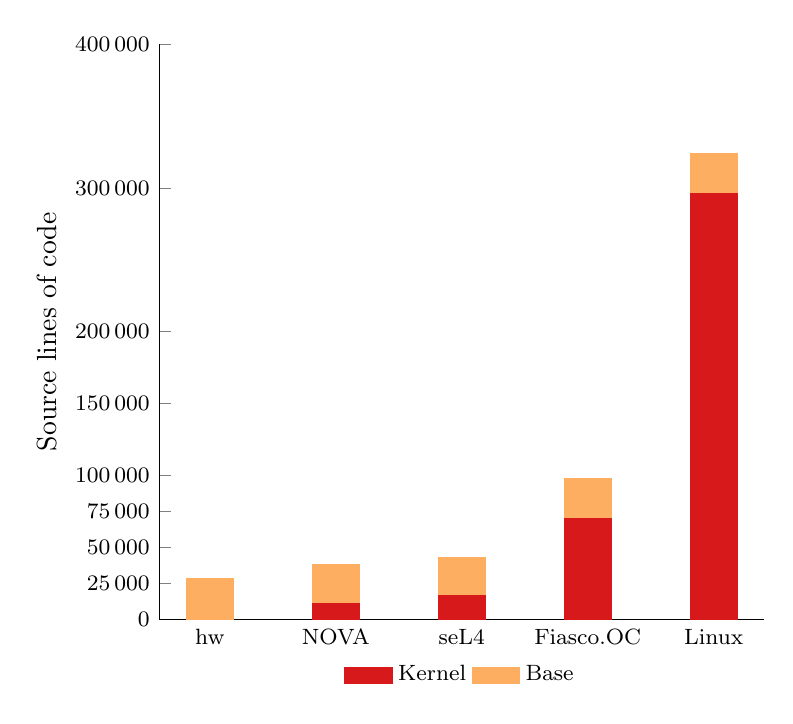
\begin{tikzpicture}
			\begin{axis}[
			ybar stacked,
			legend style={
				legend columns=4,
				at={(xticklabel cs:0.5)},
				anchor=north,
				draw=none
			},
			xtick=data,
			axis y line*=none,
			axis x line*=bottom,
			tick label style={font=\footnotesize},
			legend style={font=\footnotesize},
			label style={font=\footnotesize},
			ytick={0, 25000, 50000, 75000, 100000,
				150000, 200000, 300000, 400000},
			width=.85\textwidth,
			bar width=6mm,
			ylabel={Source lines of code},
			xticklabels={hw, NOVA, seL4, Fiasco.OC, Linux},
			ymin=0,
			ymax=400000,
			area legend,
			x=16mm,
			scaled y ticks=false,
			y tick label style={/pgf/number format/fixed, /pgf/number format/1000 sep = \thinspace},
			ylabel near ticks
			]
			\addplot[findOptimalPartition,fill=findOptimalPartition] coordinates
			{(0,0) (1,10944) (2, 16485) (3, 70210) (4, 295741)};
			\addplot[storeClusterComponent,fill=storeClusterComponent] coordinates
			{(0,28288) (1,27227) (2, 26807) (3, 27520) (4, 28300)};
			\legend{Kernel, Base}
			\end{axis}  
			\end{tikzpicture}
			\caption{Trusted computing bases}
			\label{fig:tcb}
		\end{figure}
	
	\chapter{Conclusion}
	
		This thesis shows that it is possible to create a generic interface on Linux to run drivers in the user space.
		It also shows that this is possible to do this by using a component based user land, such as the Genode OS Framework \citep{genode}.
		
		Two basic hardware access mechanisms have been ported to Linux.
		The evaluation showed that even though the implementation is not yet stable the concepts are working.
		It was possible to run unaltered Genode drivers on Linux and to create an interface that sufficiently generic to overcome the need of driver specific adaptions to the kernel.
		
		On the other hand it showed the conceptual hindrances of using a monolithic kernel in such a way.
		The best example for this is the \texttt{platform\_info} described in section \ref{pinfo} in combination with regular files being used as read only memory sessions.
		The usage of a symlinked device file and the manual manipulation of an inode by the module are merely a hack than a robust solution.
	
		\section{Future work}
		
		To be a usable solution for development and production the implementations in this concept need to reach a stable state.
		The current workarounds, that create memory leaks, need to be replaced with proper fixes.
		Also it needs to be tested further on real hardware and the issues that arose on the ThinkPad X260 require an investigation.
		With the testing of more complex drivers performance gets more important.
		Especially interrupts are often time critical and require a low latency.
		
		A further important point is the integration into Genodes build system.
		While some of it has already been done it is still unfinished.
		At the state in this thesis selecting between Genode on a bare Linux kernel and on the host system requires changes at multiple points.
		These are for example the build configuration and the Linux specific implementation of core.
		Reducing this to a switch in the build configuration is required use the results of this theses productively.
		
		The Linux kernel itself should be stripped down further.
		First of all many drivers inside the kernel already collide with their user space counterparts such as both ACPI implementations.
		Secondly the goal is to reduce the kernels complexity as far as possible.
		To achieve this any functionality that is not required needs to be removed including usually always available interfaces such as \texttt{sysfs} \citep{sysfs} and \texttt{procfs} \citep{procfs}.
		The Linux Kernel Tinification project \citep{tiny} has done some work in that direction.
		Even though their goal it to create small kernel binaries for embedded platforms and not the reduction of complexity this work is a starting point for a further microkernelization of the Linux kernel.
	
	\bibliographystyle{unsrtnat}
	\bibliography{sources}
	
\end{document}
